% !TeX root = ../../../main.tex

A crucial ingredient in the derivation of our results
is the determination of the 3\fns intrinsic
charm \pdf starting from the 4\fns, which requires the inversion of the matching
conditions implementing the 3\fns to 
the 4\fns transformation.
%
This inversion is not available in the open-source NNPDF
code~\cite{NNPDF:2021uiq} and it is performed here by means of a novel code
for QCD evolution, 
 \textsc{\small EKO} (Evolution Kernel Operators), that we use to take the
 \pdf set determined at the reference scale $Q_0$ and evolve it to a
 matching scale $Q_c$ where it is transformed to the 3\fns.
%
Here we provide a brief summary of \textsc{\small
EKO}, some details of the way the direct and inverse matching
conditions are implemented, and some benchmarks between \textsc{\small
EKO} and other existing QCD evolution codes, including the  \textsc{\small
APFEL}~\cite{Bertone:2013vaa} evolution code that is used by the
NNPDF code.
\textsc{\small EKO} is written in \textsc{\small Python} and is available
open source from its \textsc{\small GitHub} repository
\begin{center}
\url{https://github.com/N3PDF/eko}
\end{center}
A more detailed description of the code can be found
in its online documentation
\begin{center}
\url{https://eko.readthedocs.io/en/latest/}
\end{center}
as well as in a dedicated publication~\cite{Candido:2022tld}.

The scale dependence of \pdfs in QCD is determined by solving a set
of coupled integro-differential equations (evolution equations) in two
variables $x$ (momentum fraction) and $Q$ (scale) on which \pdfs depend.
Two families of approaches are commonly used in order to this purpose.
%
One possibility is to treat the (integral) dependence on $x$ of the
\pdfs and evolution kernels by
sampling it on a grid of points.
%
This is the strategy adopted by, among others, the  \textsc{\small APFEL}~\cite{Bertone:2013vaa},
\textsc{\small HOPPET}~\cite{Salam:2008qg},
and \textsc{\small QCDNUM}~\cite{Botje:2010ay} evolution codes.
%
An alternative possibility is to perform an integral transform (Mellin
transform) with
respect to $x$ thereby turning the integro-differential equations into
coupled ordinary differential equations. These can then be solved
analytically, but the integral transform has to be inverted numerically
to arrive at a final result.
%
This approach is adopted by \textsc{\small PEGASUS}~\cite{pegasus} as well as by the
internal \pdf evolution code \textsc{\small FastKernel} used in earlier NNPDF analyses
and described in~\cite{DelDebbio:2007ee,Ball:2008by,Ball:2010de}.
%
One limitation of \textsc{\small PEGASUS} is that it requires the analytic
computation of the Mellin transforms of
the \pdfs, which is generally not possible, specifically if \pdfs are
parametrized as neural networks.
%

This restriction is bypassed in \textsc{\small FastKernel} by transforming only the
evolution kernel (i.e.\ the evolution operator, solution of differential
equations, evaluated on a given interpolation basis), which can be then
convoluted with the $x$-space \pdfs at the input evolution scale $Q_0$.
Following a similar strategy, \textsc{\small EKO}
solves evolution equations in Mellin space and then produces \pdf-independent
evolution kernel operators (EKO) which can be convoluted with input 
\pdfs.
%
Variable flavor number scheme evolution (VFNS) is implemented in \textsc{\small EKO}, with
the possibility of freely choosing the value of the matching scales
$Q_{h}$ between the $N$-flavor number scheme (NFNS) in which heavy quark $h$
is not included in QCD evolution, and the $(N+1)$-flavor number
scheme in which it is included.
%
Schematically, for evolution between $Q_0$ and $Q_1$ if no matching
scales are crossed $\left(Q_{h}^2 < Q_0^2 , Q_1^2 < Q_{h'}^2\right)$ one has:
\begin{equation}
\label{eq:ic/EKO1}
{\mathbf{f}}^{(n_f)}(Q^2_1)= {\mathbf{E}}^{(n_f)}(Q^2_1\leftarrow Q^2_0) \otimes {\mathbf{f}}^{(n_f)}(Q^2_0) \, ,
\end{equation}
where
${\mathbf{E}}^{(n_f)}$ is the  NFNS \textsc{\small EKO},
and $\otimes$ is the Mellin convolution operation. Note that \textsc{\small EKO}
can perform both ``forward'' ($Q_0< Q_1$)  and ``backward'' ($Q_1< Q_0$)
evolution.
%
Bold quantities indicate either vectors or matrices
in the $(2n_f+1)$-dimensional flavor space.
If instead a single matching scale $Q_h$ is crossed, assuming for definiteness $Q_0< Q_1$,  
$Q_{h'}^2 < Q_0^2 < Q_{h}^2 < Q_1^2 < Q_{h''}^2$,
one has
\begin{equation}
\label{eq:ic/EKO2}
{\mathbf{f}}^{(n_f+1)}(Q^2_1)= \left[ {\mathbf{E}}^{(n_f+1)}(Q^2_1\leftarrow Q_{h}^2)  
{\mathbf{A}}^{(n_f)}(Q_{h}^2) {\mathbf{E}}^{(n_f)}(Q_{h}^2\leftarrow Q^2_0) \right] \otimes {\mathbf{f}}^{(n_f)}(Q^2_0) \, ,
\end{equation}
where $\mathbf{A}^{(n_f)}(Q_{h}^2)$ is the scheme transformation
between the NFNS and (N+1)\fns, given as a perturbatively computable
series expansion in $\alpha_s$. 
%
The quantity in square parenthesis is evaluated in Mellin space and then transformed to $x$-space.
%
This procedure can be  extended to the case in which  more than
one threshold is crossed.
%
Also, the scales $Q_0$ and $Q_1$ can be ordered in any way, because both direct
and inverse scheme transformations are implemented in
\textsc{\small EKO}. Furthermore, the inverse scheme change  is implemented both
perturbatively (i.e.\ as a series expansion in $\alpha_s$ to the same
accuracy as the direct scheme change) or exactly (i.e.\ as the numerical
inverse, completely equivalent to the analytic one within the numeral accuracy
of the rest of the calculation).

If the heavy quark $h$ has no intrinsic component, then below $Q_h$
its \pdf is identically zero, and above $Q_h$ it is determined by
$\mathbf{A}^{(n_f)}(Q_{h}^2)$. If it does have an intrinsic
component, then  below $Q_h$ its \pdf is scale-independent, but nonzero.
While  \textsc{\small EKO} is currently an \nnlo code, on
top of the standard~\cite{pdfnnlo} \nnlo scheme change for this work
an \nnnlo scheme change has been implemented, based on recent higher-order computations
of the relevant operator matrix elements~\cite{Bierenbaum:2009zt,Bierenbaum:2009mv,Ablinger:2010ty,Ablinger:2014vwa,Ablinger:2014uka,Behring:2014eya,Blumlein:2017wxd,Ablinger_2014,Ablinger:2014nga}
and the work of~\cite{zanoli}.

The  \textsc{\small EKO} implementation of QCD evolution has been
benchmarked against the Les Houches \pdf evolution
benchmarks~\cite{Dittmar:2005ed,Giele:2002hx} and with
\textsc{\small APFEL} and \textsc{\small PEGASUS},
finding excellent agreement beyond the per-mille level.
%
The implementation of the  matching conditions
has been benchmarked up to \nnnlo against the independent \textsc{\small Mathematica}-based calculation 
presented in~\cite{zanoli} finding also good agreement.
%
To illustrate some of these benchmarks, Fig.~\ref{fig:ic/EKObench} displays
the absolute and relative difference between \textsc{\small EKO},
\textsc{\small APFEL}, and \textsc{\small PEGASUS}
for \nnlo VFNS evolution
carried out
following the settings of~\cite{Dittmar:2005ed,Giele:2002hx}.
%
A toy \pdf set at $Q_0=\sqrt{2}$ GeV is evolved up to $Q=100$ GeV
for equal values of the factorization and renormalization scales, $Q_f=Q_r=Q$.
%
We show as representative results those corresponding to
the  total valence quark  $V$ 
and the quark singlet $\Sigma$ distributions.
%
Excellent agreement is found, in particular
with \textsc{\small PEGASUS} which also perform QCD
evolution in Mellin space, with relatively differences
at most at the $\mathcal{O}\left( 10^{-4}\right)$ level.
%
A similar level of agreement is found
for the gluon and for the other quark \pdf combinations.

%%%%%%%%%%%%%%%%%%%%%%%%%%%%%%%%%%%%%%%%%%%%%%%%%%%%%%%%%%%%%%%%%%%%%%
\begin{figure}[t]
    \begin{center}
        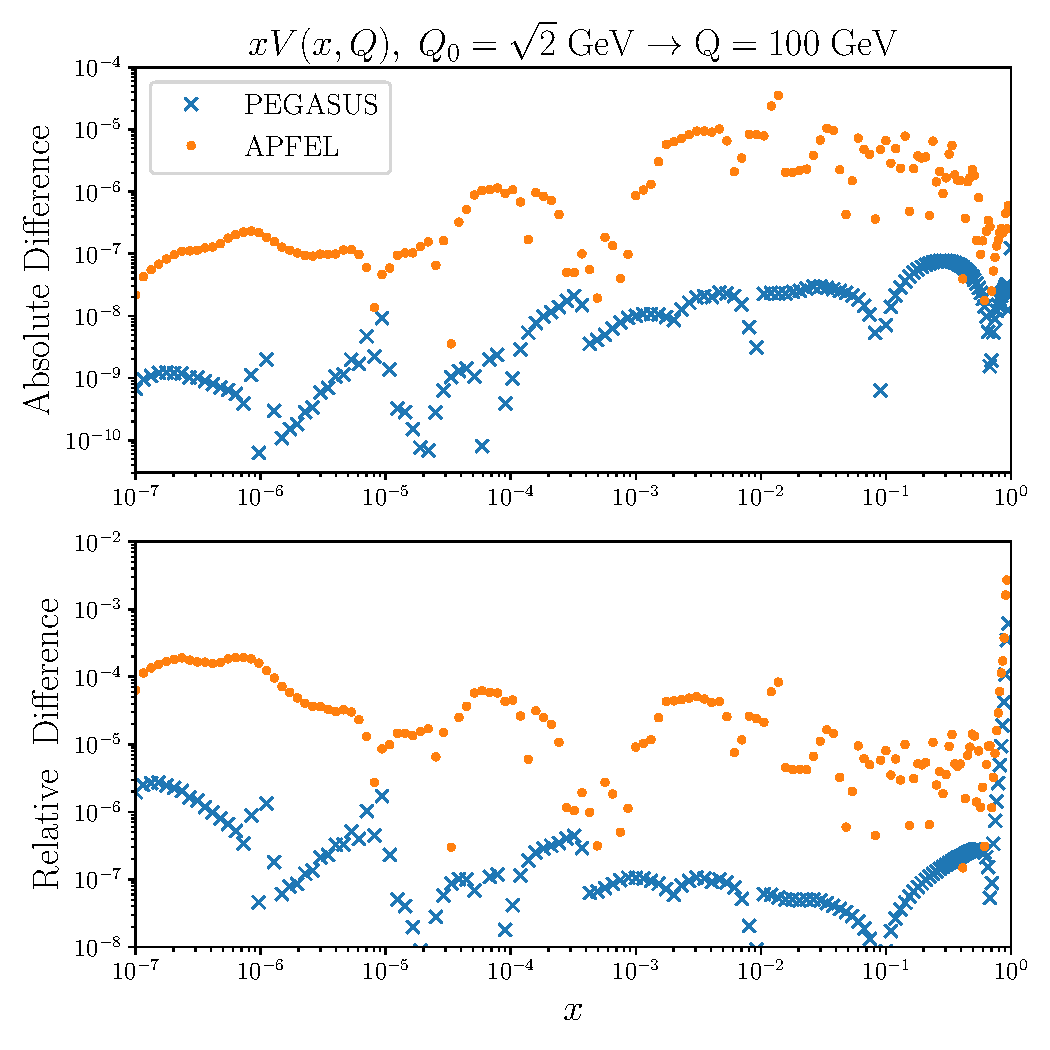
\includegraphics[width=0.47\linewidth]{ch-ic/eko_bench_V.pdf}
        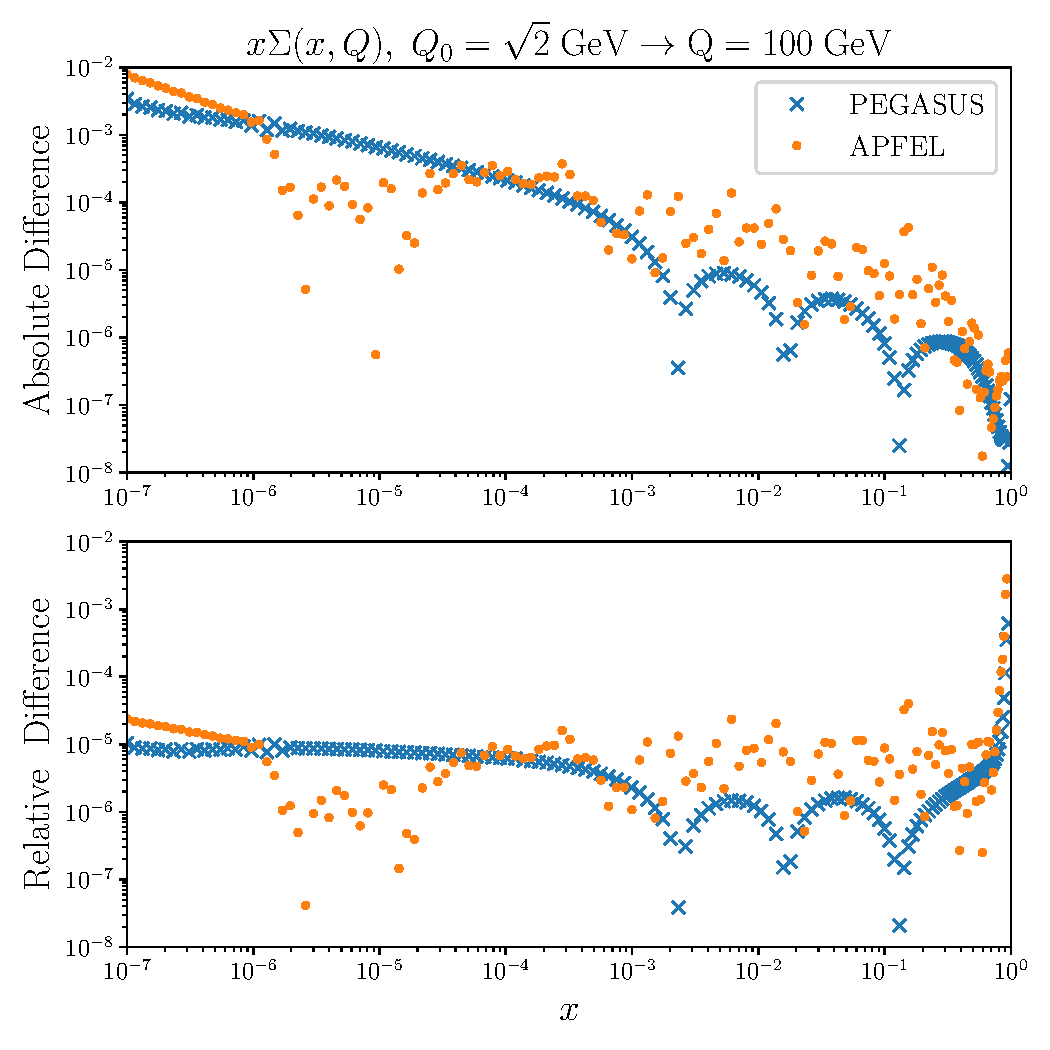
\includegraphics[width=0.47\linewidth]{ch-ic/eko_bench_S.pdf}
        \caption{\small Absolute (upper) and relative (bottom) differences between 
        the outcome of \nnlo QCD evolution
        as implemented in
        \textsc{\small EKO} and the
        corresponding results from \textsc{\small APFEL} and \textsc{\small PEGASUS}.
We adopt the settings of the Les Houches \pdf evolution benchmarks: we
consider  VFNS evolution from $Q_0=\sqrt{2}$ GeV up to $Q=100$ GeV,
and we show  results for the total valence quark distribution $V$ (left)
and the quark singlet distribution $\Sigma$ (right).
      \label{fig:ic/EKObench} }
    \end{center}
\end{figure}
%%%%%%%%%%%%%%%%%%%%%%%%%%%%%%%%%%%%%%%%%%%%%%%%%%%%%%%%%%%%%%%%%%%%%%
